\section{Main elements of the user interface}
\label{sec:user_interface}
This section gives an overview of the main user interface elements and features of RKWard.
For a use-case oriented example of an RKWard session, see Section~\ref{sec:using_RKWard}.

The default layout of the main application window is divided into five
parts, as depicted in Figure~\ref{fig:main_window}. While many aspects
of the GUI can be customized by the user, for simplicity we will
describe the default appearance of RKWard in the present section. The
top of the window is occupied by menu bar and toolbar (Figure~
\ref{fig:main_window}A). The content of both bars is partially context
sensitive, e.\,g., the Edit menu will offer
one set of actions when the current document window is a data editor,
and another set of actions for a \proglang{R} script
editor window. To ease orientation, all top level menus remain
persistent, even if no actions are available for that menu in the
current context. The menu bar of the main window is also the central
access point to most data import, manipulation, analysis, and
visualization features (see Section~\ref{sec:analyzing_data}) for which RKWard provides a GUI
interface.

\begin{figure}[htp]
 \centering
 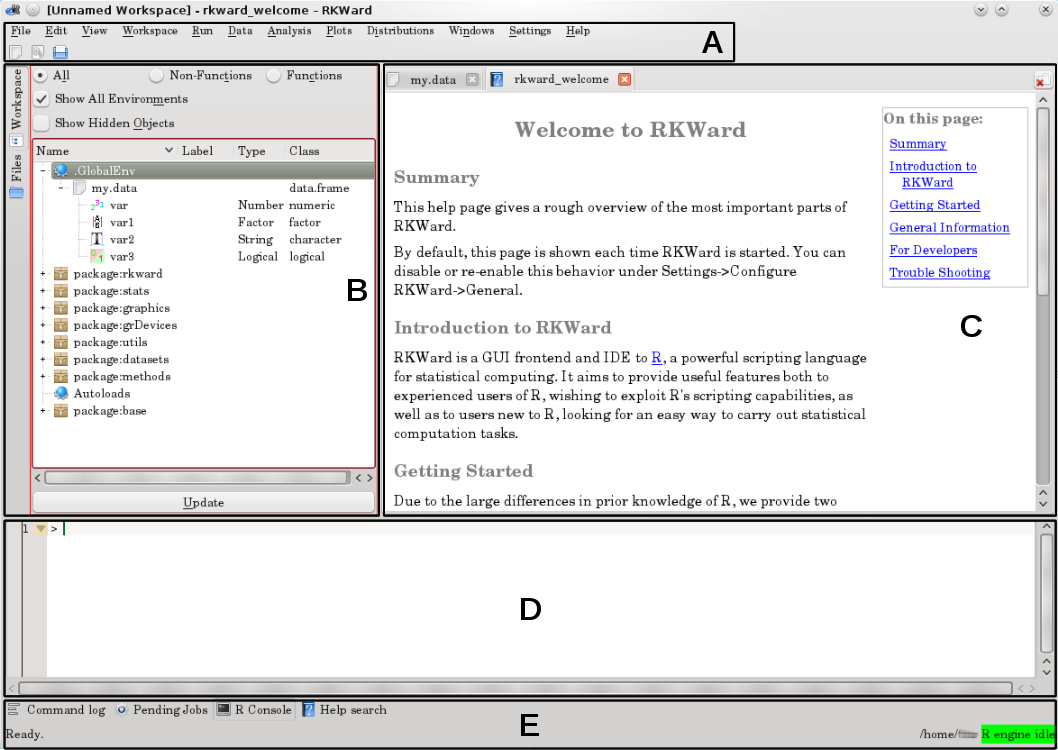
\includegraphics[width=15.446cm,height=10.949cm]{../figures/main_window.png}
 \caption{Default RKWard main window after start up. 
A) Menubar and toolbar, B) navigator element, C) editor, output, 
and data management. D) embedded \proglang{R} console. 
E) In addition to the menu bar at the top A) toolbar buttons 
on the bottom of the main window give quick access to the command log, 
running jobs, an \proglang{R} console, and the \proglang{R} help. 
RKWard main window. Panels B) and D) can be resized or collapsed. The navigator element B)
presents detailed information (e.\,g., type, class) about objects and their properties.}
 \label{fig:main_window}
\end{figure}

A status bar is shown at the bottom of the window. It displays (from
right to left) the status of the \proglang{R} engine (busy or idle), the
current working directory, and a multi purpose region for additional
information on some menu items and other GUI elements, visible when
hovering the mouse pointer over them.

The central area is divided into a document view area
(Figure~\ref{fig:main_window}C) and two panel subwindows
(Figure~\ref{fig:main_window}B and D). The panels can be resized or moved to
another edge of the central area independently. All panels can be
toggled by mouse or keyboard shortcuts. When a panel is closed, the
document view area (see below) is automatically re-sized to take up the
free space.

The left panel (Figure~\ref{fig:main_window}B) contains a file browser (see Section~\ref{sec:further_tool_windows}) and a
workspace browser (see Section~\ref{sec:workspace_browser_object_viewer}) by default. The
bottom panel (Figure~\ref{fig:main_window}D) contains the tool windows, namely, Command
log (Section~\ref{sec:further_tool_windows}), Pending Jobs (Section~\ref{sec:further_tool_windows}), \proglang{R} Console
(Section~\ref{sec:using_R_console}), and Help Search (Section~\ref{sec:help_system}).

The remainder of the central area (Figure~\ref{fig:main_window}C) is a single row Tab Document
Interface (TDI) for different documents. Early uses of TDIs date back to 1988 and are
widely applied nowadays \citep{Hopkins2005, MDN2010,
KimLutteroth2010}. Currently, the supported types of
documents are object summaries (Section~\ref{sec:workspace_browser_object_viewer}), 
script editors (Section~\ref{sec:code_editor}), spreadsheet-like data editors 
(Section~\ref{sec:spreadsheet}), results output (Section~\ref{sec:results_output}), 
help pages (Section~\ref{sec:help_system}), and also
\proglang{R} onscreen graphics devices (Section~\ref{sec:technical_graphics}). 
The order of tabs can be conveniently re-arranged
using drag \& drop.

Both document windows and tool views can be detached and re-attached from the main
window as independent windows, managed by the window manager. This feature allows to 
conveniently work with multiple documents
at the same time, e.\,g., scripts or data editors. On{}-screen
graphics device windows are created detached by default, but can 
be attached to the document view area of the main window.

Windows can be shown (or toggled) using a mouse device with point \&
click, as well as using a series of keyboard shortcuts (defined by
default) for switching between the different tool and document windows.
Key bindings can be configured from the GUI via ``Settings$\rightarrow$Configure Shortcuts''. 
However, for technical reasons only the shortcuts of currently active components 
will be listed. Thus, for example, to
configure data editor shortcuts, one has to open a data editor first and
then to select ``Settings$\rightarrow$Configure Shortcuts''. Since RKWard relies on the 
\proglang{KDE} SC editor component,
shortcuts for the script editor (Section~\ref{sec:code_editor}) are managed separately via 
``Settings$\rightarrow$Configure Editor$\rightarrow$Shortcuts''. On most systems, it is also
possible to configure shortcuts by right-clicking on the respective
menu item.

The choice of available actions on the tool bar can be
configured via ``Settings$\rightarrow$Configure Toolbars''. Further, it is possible to add and remove sets
of data manipulation and analysis features from the GUI, using
``Settings$\rightarrow$Configure RKWard/Plugins''.

\subsection{Workspace browser and object viewer}
\label{sec:workspace_browser_object_viewer}

The workspace browser allows to view
and manipulate \proglang{R} objects, similar
to a regular file-system browser. This includes both, user objects
(data, functions, environments) in \code{.GlobalEnv} and non-user objects in other environments in the
\proglang{R} search path (typically,
\proglang{R} package environments). Objects are shown
in a hierarchical tree structure. For instance, an object of class
\code{list} can be expanded to show all contained objects 
by clicking on the $+$ symbol left of the object name.
The basic type of each object is indicated by specific icons. Further
information on each object can be seen by hovering the mouse
pointer over the respective icon. A tooltip window will appear,
including information such as dimensionality or function arguments,
depending on the type of object. Further, objects inside \code{.GlobalEnv} can be
removed, renamed, and edited from the context menu.

Literally hundreds or even thousands of objects are present in a typical
\proglang{R} session. This can be overwhelming at
first, therefore, the workspace browser has options to show only a certain
subset of objects, e.\,g., only functions or only data objects, including
or excluding hidden objects (object names starting with a 
``.''), or showing only the contents of \code{.GlobalEnv} as
opposed to all environments in the search path.

Several actions are available from a context menu (after right-clicking
on the object names), depending on the type of object. These allow to search the
\proglang{R} help for information on that object, to
open a window with detailed information on the object, to delete, rename or copy the object to a new symbol name, or to
copy it to \code{.GlobalEnv}. Further, the context menu allows to open
supported types of objects for editing (see Section~\ref{sec:spreadsheet}; currently, only
\code{data.frame}s can be edited, and only while they exist in \code{.GlobalEnv}). 
Selecting ``View'' from the 
context menu opens a new window in the
document area, containing basic information on the object as well as 
tabs which show the output of
\code{print()} and \code{summary()} calls.

An object list similar to the workspace browser (but showing only 
\code{.GlobalEnv} by default) is also used in several places for the
selection of objects to work with, e.\,g., in an analysis plugin (see Section~\ref{sec:analyzing_data}).


\subsection{Code editor}
\label{sec:code_editor}

RKWard comes with an advanced
\proglang{R} script editor, based on the
\proglang{KDE} Advanced Text Editor component
(\url{http://kate-editor.org/}). Features of this
editor include syntax highlighting (both on screen and in printouts; for
\proglang{R} and many other script types), code
folding, block-wise indentation adjustments or commenting, automatic
brackets, search and replace with plain text or regular expressions,
and many more. The editor automatically saves snapshots of the
currently edited files at configurable intervals.

For interaction with \proglang{R}, the editor has
predefined shortcuts (and toolbar icons) for submitting the current line, the current 
selection, predefined blocks, or the entire document to the
\proglang{R} engine for evaluation. It also 
offers object-name completion and function argument hinting (Figure
\ref{fig:code_hinting}A and B) based on the objects present in
the \proglang{R} workspace\footnote{The object-name
completion and function argument hinting features in RKWard predate the
inclusion of similar features into the core
\proglang{R} distribution. For this reason, they are
technically based on different mechanisms.}. A further feature specific
to the \proglang{R} language is the
``Paste Special'' action, which allows to
paste the clipboard content (e.\,g., from a separate spreadsheet
application) as a single string, vector, or matrix, suitable
for inclusion in an \proglang{R} script, optionally
transforming it in advance (Figure \ref{fig:special_paste}).

\begin{figure}[htp]
 \centering
 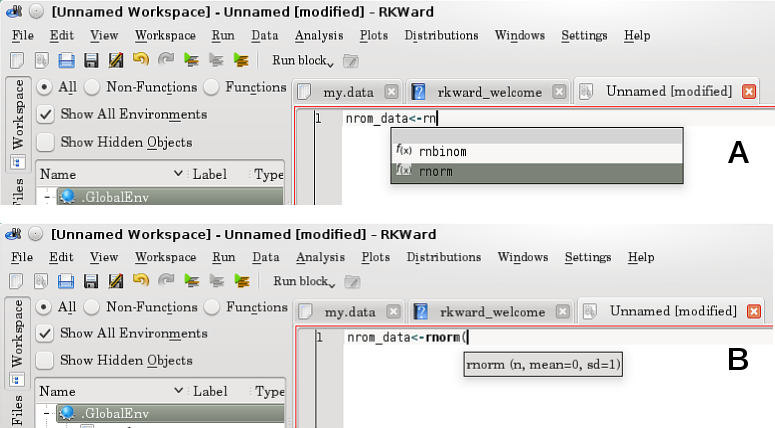
\includegraphics[width=15.5cm]{../figures/code_hinting.png}
 \caption{Code hinting features of the script editor. The script editor is able to hint A) \proglang{R} object names
and B) function arguments.}
 \label{fig:code_hinting}
\end{figure}

\begin{figure}[htp]
 \centering
 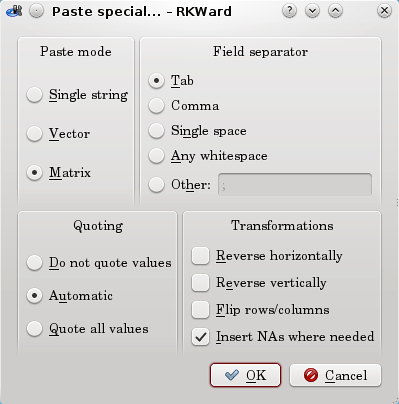
\includegraphics[width=8.042cm,height=8.143cm]{../figures/special_paste.png}
 \caption{Special paste dialog. This tool allows to paste data (e.\,g., tabular, text) from the clipboard, directly to an 
 \proglang{R} script and therefore accelerates the work process with data from different sources 
 like spread-sheet applications.
}
 \label{fig:special_paste}
\end{figure}

Script editor windows can be created by opening an existing
\proglang{R} script file from the file browser, the
``File''-menu, or by creating a new empty script. It can
also be invoked from \proglang{R}, e.\,g., using the
\code{file.edit()}, \code{file.show()}, or \code{fix()}
commands.

\subsection{Using the R console}
\label{sec:using_R_console}
For users with knowledge of \proglang{R}, RKWard provides direct access to the
embedded \proglang{R} engine in the
\proglang{R} console tool window. It is important to understand that technically this is an
emulation of \proglang{R} running in a console
session, not a real \proglang{R} session. This leads to a few subtle
differences, e.\,g., with respect to the command history feature in
\proglang{R}.

However, for most purposes RKWard's \proglang{R} console can be used exactly
like \proglang{R} running in a terminal. Adding to that, it provides many of the
features which are also available in the code editor (see Section~\ref{sec:code_editor}).
Most prominently, it supports syntax highlighting, code
folding, function argument hinting, object-name completion, and pasting
vector or matrix data directly from the clipboard.

By default, any code that is submitted to the
\proglang{R} engine from the code-editor or from help
pages, is sent through the \proglang{R} console.
However, it can be configured to the submitted in the background,
instead.
For further technical details, see Section~\ref{sec:technical}.

\subsection{Spreadsheet-like data editor}
\label{sec:spreadsheet}

Historically, one of the earliest
features of RKWard is a built-in spreadsheet-like data editor.
Currently, editing \proglang{R} objects of type
\code{data.frame} is possible. In contrast to the \code{data.frame} editing shipped
with the \proglang{R} core distribution, this editor
gives the illusion of ``in-place'' editing of data. New \code{data.frame}s can
be created and opened from the GUI, and existing objects can be opened
for editing from the workspace browser. For opening objects from
\proglang{R} code, the function \code{rk.edit()} can be used.
Figure \ref{fig:data_editors} shows multiple \code{data.frame}s open for editing.

\begin{figure}[htp]
 \centering
 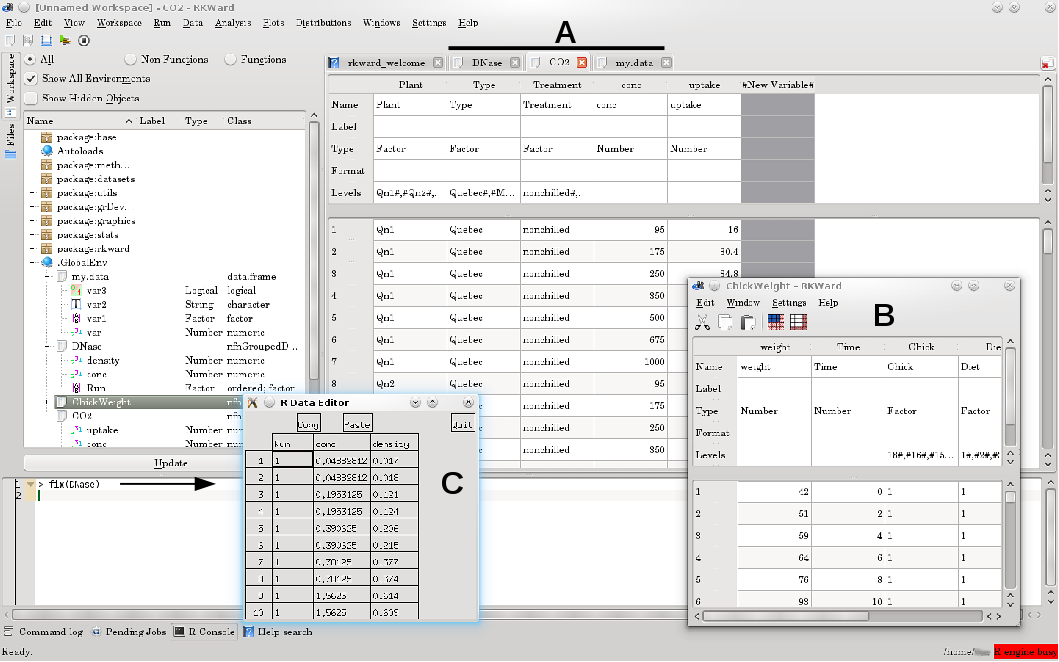
\includegraphics[width=15.5cm]{../figures/data_editors.png}
 \caption{RKWard with several \code{data.frame}s in use at the same time. A) 
  One \code{data.frame} is opened for editing in the main window. Further 
  two documents (\code{data.frame}s) are opened in the background. 
  B) A second \code{data.frame} is opened as detached window. 
  C) \proglang{R}'s standard data editing features (e.\,g., \code{fix()}, \code{edit()}) 
  are also usable within an RKWard session. In this example \code{fix(DNase)} 
  was invoked from the console (arrow).}
 \label{fig:data_editors}
\end{figure}

Meta-data on each column of a \code{data.frame} (i.\,e., name of the column, data
type, and potentially data labels) is shown in the upper portion of
the data editor, and can be manipulated there, while the data itself is
shown in the lower portion. The upper portion can be hidden using a
slider, to save space for the display and editing of actual data.
Similarly, an editable column showing the row names of the \code{data.frame}
can be shown or hidden separately from the data.

For columns of type \code{factor}, factor levels can be edited by double-clicking on the
``Levels'' row of the meta information. Levels can also be assigned to other types of
variables, but only for consecutive integer values. These levels will
be displayed instead of the underlying value, if applicable. Each
column can also be assigned an arbitrary descriptive
``Label'', which is stored in
\proglang{R} as an attribute of the column.

Contrary to many other editors, the data editor in RKWard does not
automatically convert data types of columns. For instance, if a
non-numeric string is entered into a cell of a numeric column, the data
type of the column remains numeric, and the entered value is
highlighted in red. Internally, the invalid cell is set to \code{NA}.
The entered value is stored separately, in an attribute of the column.
The rationale for this approach is that it offers protection against
accidental, and probably undetected, conversion of data types. The
user can manually convert the storage mode of a column by simply
selecting a different data type in the ``Type'' row of the meta information.

The data editor supports insertion and deletion of rows or columns at 
arbitrary positions. Rows (columns) can also be added at the bottom 
(right) by simply entering data into the trailing row (column) shown in
gray. Copy \& paste is supported, where the area affected by paste
operations can optionally be constrained to the selected region, or to
the dimensions of the table. The data editor can also be set to read-only
mode to examine data objects.

In the context of data editing, it is noteworthy that
RKWard supports working with multiple objects simultaneously, rather than
limiting actions to a single active \code{data.frame}, as with e.\,g., \pkg{Rcmdr} or
\pkg{DeduceR}. Given this non-modal interface design, multiple data editor
windows can be opened at once (Figure \ref{fig:data_editors}).

\subsection{Handling, manipulating, and analyzing data}
\label{sec:analyzing_data}

Dealing with data -- i.\,e., importing, transforming, filtering, analyzing, and visualizing  --
is the core strength of \proglang{R}, and one central goal of
RKWard is to make the most of this functionality available to a broader
audience by providing it in the form of easy to use GUI dialogs. Since
the data handling functionality itself is provided by
\proglang{R} and its numerous add-on packages, this
can basically be accomplished by defining GUI dialogs, generating
\proglang{R} code according to the settings made in
the GUI, and have the generated code evaluated by the
\proglang{R} engine. 
This general pattern, implemented as plugins, is the
basic recipe for most of the functionality provided by RKWard
(see Section~\ref{sec:technical_plugins} for details). 
Note that on purpose, RKWard does not have its
own file format for data import and export. That is, it is possible
to import data from several sources (see below) or to save and load
\proglang{R} workspaces.
For
the purpose of this article we will look at the standard
elements of data handling functions by example of importing CSV
(comma-separated values) data.

At the time of this writing, RKWard provides support for importing SPSS, 
Stata, and ``delimited text'' data. Internally, RKWard
relies on \proglang{R} packages for certain sets of
data which were already described elsewhere
\citep{Murdoch2002}. Of course, further formats can
also be imported using copy \& paste (see Sections~\ref{sec:code_editor} and \ref{sec:spreadsheet}), or by
manually entering appropriate \proglang{R} commands in
the \proglang{R} console (Section~\ref{sec:using_R_console}). To import CSV
data, select ``File$\rightarrow$Import format$\rightarrow$Import Text$\rightarrow$CSV''
data from the menu. This will open the dialog shown in
Figure~\ref{fig:import_data}A. The central area of this dialog provides 
options to control the import. The 
``File name'' field is highlighted, to indicate that
it is required to specify a file before the dialog can proceed.
Further options are available from the tabbed pages of the central area.

The right-side area is common to all data handling
dialogs. Here the ``Submit button'' is used
to start the import action. It is enabled once all required
settings have been made, i.\,e., in this case a file name has been
selected. The ``Close'' button will close the
dialog without taking any action.

The bottom area optionally shows the \proglang{R}
code corresponding to the current settings, and which will be run
upon pressing the ``Submit button'' (see Section~\ref{sec:importing_data} for generated \proglang{R} code). 
The code display is hidden by default and can be revealed using
the ``Code'' button. This 
generated code display is updated dynamically as the user changes settings, allowing
to see the effect of each change instantly.

Most data handling functions will produce some output, which is
sent to the output window. From there it is possible to repeat the
action by clicking on the ``Run again''-link
(see Section~\ref{sec:results_output}).

\subsection{Graphics window and plot previews}
\label{sec:plot_previews}

For plotting, RKWard relies on the graphics capabilities provided by
\proglang{R}. All \proglang{R}
devices, including on{}-screen devices, can be used in the regular way.
However, for the \code{X11()} and \code{windows()} devices, RKWard adds a menu
bar and a toolbar to the device windows (on the MS Windows platform,
replacing the default menu bar provided by the device). The menu
bar and toolbar give access to a number of different functions,
including GUI dialogs for exporting the current plot,
and adding a grid to an existing plot 
(works on only certain types of plots). Further, a history mechanism is provided,
which stores most created plots automatically and allows to navigate
back to earlier plots (Figure \ref{fig:plot_history}). 
The history is available as a drop down list of the plot calls as well as using typical ``back''
and ``forward'' buttons on the toolbar.
The maximum number
of plots to record, as well as the maximum size of each individual plot,
is configurable from the settings menu. This plot history is shared
between the open on{}-screen device windows, yet they behave
independently. For example, if multiple devices display the same
plot, any modification (including deletion) of the plot on one device
renders its instances on other devices as ``new'' and hence can be added
back to the plot history. In addition, duplicating or closing a device
window records any unsaved plots to the history.

\begin{figure}[htp]
 \centering
 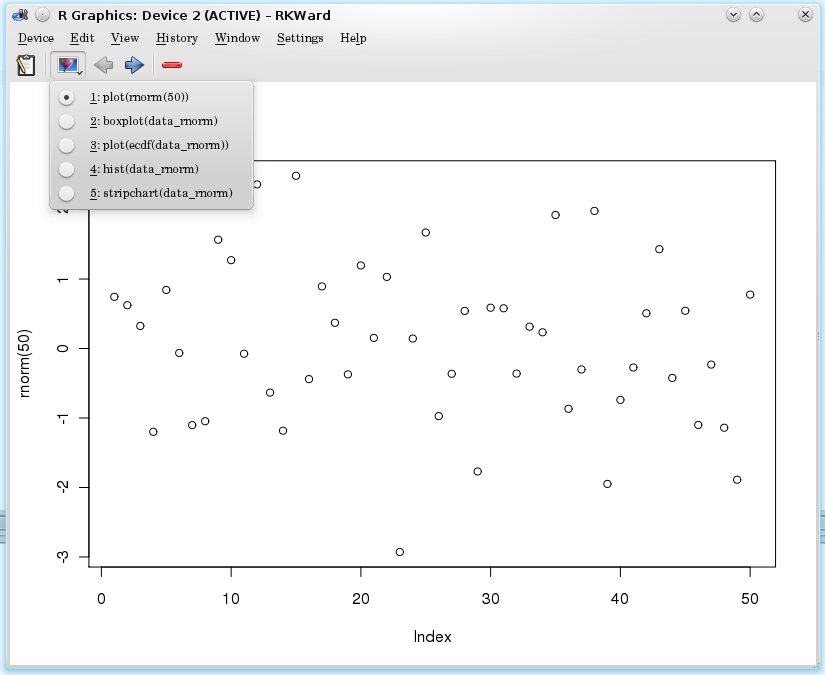
\includegraphics{../figures/plot_history_cropped.png}
 \caption{On{}-screen graphics device window in RKWard. The plot history is 
  available as a drop-down list, allowing to jump directly to a previous 
  plot. In this example, five different plots were performed on the same data 
  set of a random sample (\code{rnorm()}). The plot can be 
  selectively exported as described in Figure~\ref{fig:boxplot2} via ``Device$\rightarrow$Export''.
}
 \label{fig:plot_history}
\end{figure}

Further, RKWard provides access to different plotting functions using GUI dialogs,
available from the ``Plots'' menu. Wherever appropriate, RKWard supports a ``plot
preview'' feature. If the ``Preview'' box of
the respective dialog is checked (c.\,f., Figure \ref{fig:boxplot1}), a device window is opened, which
shows the plot as it would be created with the current settings. The
preview is updated automatically as the user makes changes, allowing to
see the effect of each setting instantly\footnote{The preview is
updated asynchronously to keep the GUI responsive; see Section~\ref{sec:technical_graphics}.}. For example, the CLT plugins
under the ``Distributions'' menu can be very helpful to dynamically ``show''
the convergence in distribution while teaching. For the sake of simplicity, such preview plots are not added to
the history.

\subsection{Results output}
\label{sec:results_output}

While all basic mechanisms of
capturing and documenting \proglang{R} output can also
be used, RKWard provides a dedicated output file and a output
window for documenting the results. All GUI-driven data handling
functions (see Section~\ref{sec:analyzing_data}) write their output to this file. 
The same applies to error messages, in case a plugin fails to perform its task.
The output is presented in a journal format\footnote{Note: The font size of the output can be adjusted
from the menu. 
Since it is based on \proglang{HTML}, it is also possible to view the source code 
(see below).}. All results are presented
sequentially with the last performed task at the bottom.
It is also possible to write to the output directly from \proglang{R}
scripts by using a number of dedicated \proglang{R}
functions included in the \code{rkward} package. For the GUI-driven data handling functions, the output is
standardized to include the name of the feature, the date and time of
its execution, and other basic parameters, wherever
applicable. Further, a clickable ``Run
Again'' link is rendered below the output of each data
handling feature, which allows to invoke the same feature again with
identical parameters\footnote{In case not all parameters could be
reused, since, may be, some of the objects in
question are no longer available, the user will be notified.} (see
Figure \ref{fig:results_output}). Thus, the ``Run
Again'' feature combines the documentation of the result
with an automated way to conduct the same analysis again on new
data, providing benefits similar to, for example, the automated report generation
available from \pkg{RreportGenerator}\footnote{The application generates automatic
reports from routine statistical analysis in bioinformatical
applications.} \citep{RaffelsbergerW2008}.

\begin{figure}[htp]
 \centering
 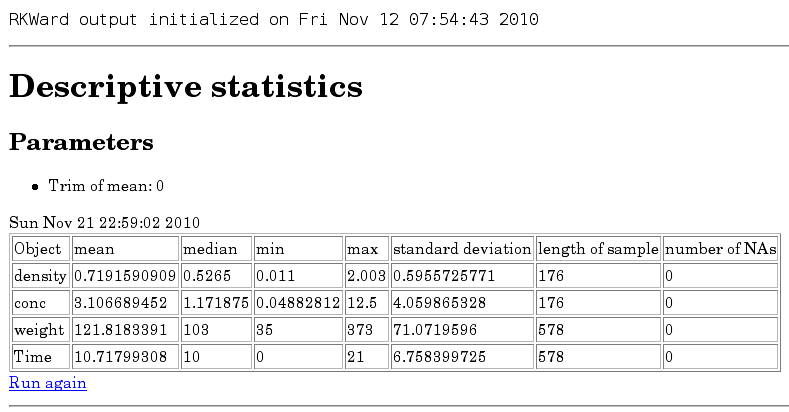
\includegraphics[width=15.5cm]{../figures/results_output_cropped.png}
 \caption{Sample contents of the output window. DNase data of the \pkg{data} package was used. 
  Standard elements of plugin output include  a standardized header, and a 
  ``Run again''-link, which allows to repeat the analysis with identical or 
  similar parameters.}
 \label{fig:results_output}
\end{figure}

The formatting of the output is kept to a minimum. In particular,
RKWard is very reluctant to round numerical results for the sake of a
pretty output. Rather, the focus is on making the results easily
accessible for further processing, typically in a dedicated word
processor. Output is based on
\proglang{HTML} (hypertext markup language), and the raw
\proglang{HTML} file and any images therein can be directly
retrieved from a dedicated folder
($\sim\!$/.rkward, by default). It is also
possible to select and copy sections of the output directly from the
output window, and to paste them into office applications as
richly formatted text; even images and tables can be easily copied by drag \& drop. In future releases, 
it is planned to integrate RKWard
with existing office suites. This
will possibly also mean addition of different file formats such as ODF (open
document format) and technologies such as \pkg{sweave} and \pkg{odfWeave}
\citep{Leisch2002, Kuhn2006}.

Images contained in the output are stored as
PNG\footnote{\url{http://www.libpng.org/pub/png/}} by
default, but JPEG\footnote{\url{http://www.jpeg.org/index.html}} and
SVG\footnote{\url{http://www.w3.org/Graphics/SVG/}}
can also be used. Similarly, the size of 
images can be configured by the user. It is expected that SVG will
become the default output format eventually, but currently some SVG
files produced by \proglang{R} are not properly
rendered by older supported versions of the
\proglang{KDE} libraries.

\subsection{Package management}
\label{sec:package_management}
The number of \proglang{R} packages available from CRAN (the comprehensive \proglang{R} archive
network), Omegahat\footnote{\url{http://www.omegahat.org/}} and Bioconductor \citep{Gentleman2004} has grown exponentially since \proglang{R}\, 1.3
(2001) to \proglang{R}\, 2.7 (2008) \citep{Fox2008, Ligges2003, Visne2009}. RKWard
utilizes functionality from a growing number of these packages, but avoids
making the installation of all supported packages a pre-requirement to using
RKWard at all. Only once a not yet installed package is required to conduct a certain
action, a package management dialog is invoked automatically, which allows to
download and install the package from a repository such as CRAN. The package
management dialog can also be invoked manually from the menu
(``Settings$\rightarrow$Configure Packages'') for installing new or updating existing \proglang{R}
packages. The underlying package management technology is that of \proglang{R}
\citep{Ligges2003, Ripley2005}.

RKWard supports installing packages to any user writable location. If no current
library location is user writable, RKWard offers to create a new one. 
On UNIX systems, interactively acquiring root privileges for
installation to the system-wide libraries is also supported. If used to
update already installed packages, the user can choose to either
update all packages at once, or only the selected ones. The installation process
itself can be monitored at the interface for error tracking. At the time of this writing, RKWard has no
built-in tools for the interactive exploration of \proglang{R} packages. However, it is
possible to invoke external helpers \citep{Zhang2004}.

\subsection{Further tool windows}
\label{sec:further_tool_windows}

The file browser tool window can be
used to open supported file types (e.\,g., \proglang{R}
scripts, \proglang{HTML} files) inside the main RKWard
window. For unsupported file types (such as PDF), the
systems default external applications are used.

The command log window contains a log of the commands that have been
evaluated by the \proglang{R} engine, and any output
produced by these commands. By default, the log shows only commands
which have been entered by the user or directly correspond to user
actions, but it can be configured to include commands which are run for
RKWard's internal purposes such as keeping the workspace browser up
to date.

Commands can be submitted while the \proglang{R} engine
has not yet started, or while another lengthy calculation is still
in progress. In these cases commands are placed into a queue first, and
executed as soon as the \proglang{R} engine becomes
available. The ``pending jobs'' window lists current \proglang{R} commands waiting for
evaluation by the \proglang{R} engine. While this
window is mostly of interest to application developers for diagnostic
purposes, it can also be used to interrupt selected commands.

\subsection{Help system}
\label{sec:help_system}
%Help on \proglang{R}
%or RKWard are easily available and accessible through an arbitrary number of document
%windows. These allow to browse \proglang{R} manuals in
%\proglang{HTML} form, help pages on
%\proglang{R} functions and packages, help pages on
%RKWard in general, and help pages on specific GUI dialogs within
%RKWard\footnote{For technical backgound of RKWard GUI help pages 
%please refer to Section~\ref{sec:technical_plugins_defining}}. 
%All types of help can be browsed in the
%same document window, and can be cross-linked. For example, help pages for
%RKWard GUI dialogs will typically link to documentation for both
%related RKWard dialogs and the underlying
%\proglang{R} functions.

RKWard provides access to both \proglang{R}  specific and 
RKWard specific help pages seamlessly in a unified framework. 
The former includes documentation on \proglang{R} functions and packages 
and the various R manuals; while the later includes help pages on 
RKWard in general and on specific GUI dialogs\footnote{For technical 
backgound of RKWard GUI help pages please refer to Section~\ref{sec:technical_plugins_defining}.}. 
All these various types of help pages can be browsed in the same document 
window, and are appropriately cross--linked. For example, help pages for
RKWard GUI dialogs will typically link to documentation for both
related RKWard dialogs and the underlying \proglang{R} functions.
It worthwhile to note here that, the TDI interface of the document view area 
(c.\,f., Figure \ref{fig:main_window}C) allows to utilize arbitrary number of document 
windows for browsing these help pages simultaneously.

%The help system can be invoked through several actions in the
%Help menu. Help pages on RKWard dialogs can be
%accessed from the dialog itself using the
%Help button. They
%also allow starting the respective dialog by click on a link near the
%top of the page. Help on \proglang{R} specific
%functions can be invoked from the context
%menu of the workspace browser, by pressing F2 (Function
%reference) while the cursor is on a function name in the
%code editor or the \proglang{R} console, or by using
%the \proglang{R} \code{help()}
%command. In addition, a tool view is provided as an interface to the
%\code{help.search()} command in
%\proglang{R}. This allows to search all installed, all
%loaded, or specific \proglang{R} packages for a
%specified topic.

An easy way to access the help system is the ``Help'' menu. Help pages on
RKWard GUI dialogs can be accessed from the dialog itself using the
``Help'' button. An useful (``reverse'') feature here is that these pages include 
a link near the top of the page to start the corresponding GUI dialog directly.
Help on \proglang{R} specific functions can be invoked from multiple places, 
such as, the context menu of the workspace browser, by pressing F2 (function
reference) while the cursor is on a function name either in the code editor or 
in the \proglang{R} console, and of course, by using the \proglang{R} \code{help()}
command. In addition, a tool view window\footnote{Note the ``Help search'' 
tool in Figure \ref{fig:main_window}E.} is provided as an interface to the
\code{help.search()} command in \proglang{R}. This allows to search all installed, 
all loaded, and related \proglang{R} packages for a specified topic.

The help browser window is based on the \proglang{KDE}
\proglang{HTML} viewer component and supports typical
features like increasing or decreasing the font size and searching text
within a page. Additionally, \proglang{R} code inside a help
page can be sent to the \proglang{R} engine for
evaluation by selecting it and pressing F8 (or via ``Run$\rightarrow$Run
Selection'').
